\chapter{PHÂN TÍCH HỆ THỐNG}
\label{ch:system-analysis}

\section{Use Case Diagram}
\label{sec:use-case-diagram}

\subsection{Tổng quan Use Case}
\label{subsec:use-case-overview}

Hệ thống DSA Visualizer Platform phục vụ ba nhóm actor chính: Student, Instructor và Admin. Mỗi actor có các use case riêng biệt phù hợp với vai trò và quyền hạn của họ trong hệ thống.

\begin{center}
\textbf{[Use Case Diagram - System Overview]}\\
\textit{Diagram available in enhanced-diagrams/usecase-system-overview.drawio}
\end{center}

\subsection{Use Case chi tiết cho Learning Process}
\label{subsec:learning-process-usecase}

Quá trình học tập là core functionality của platform, bao gồm nhiều use case phức tạp với các interaction giữa Student và các subsystem khác nhau.

\begin{center}
\textbf{[Use Case Diagram - Detailed Scenarios]}\\
\textit{Diagram available in enhanced-diagrams/usecase-detailed-scenarios.drawio}
\end{center}

Các use case chính trong Learning Process:

\begin{enumerate}
    \item \textbf{Start Learning Session}: Khởi tạo session học tập mới
    \item \textbf{Select Algorithm}: Chọn thuật toán cần học
    \item \textbf{Study Theory}: Đọc tài liệu lý thuyết
    \item \textbf{Practice with Visualization}: Thực hành với animation
    \item \textbf{Solve Practice Problems}: Giải bài tập thực hành
    \item \textbf{Take Assessment}: Làm bài kiểm tra đánh giá
    \item \textbf{Get AI Assistance}: Nhận hỗ trợ từ AI assistant
    \item \textbf{Track Progress}: Theo dõi tiến độ học tập
\end{enumerate}

\subsection{Detailed Use Case Specifications}
\label{subsec:detailed-usecase-specs}

\subsubsection{UC001: Algorithm Visualization Learning}

\begin{longtable}{| p{3cm} | p{10cm} |}
\hline
\textbf{Use Case ID} & UC001 \\ \hline
\textbf{Tên Use Case} & Algorithm Visualization Learning \\ \hline
\textbf{Actor} & Student \\ \hline
\textbf{Mô tả ngắn gọn} & Học viên học thuật toán thông qua visualization interactive \\ \hline
\textbf{Trigger} & Học viên muốn học và hiểu thuật toán thông qua visualization \\ \hline
\textbf{Precondition} & 
\begin{itemize}
    \item Học viên đã đăng nhập vào hệ thống
    \item Hệ thống có sẵn algorithm content
    \item Browser hỗ trợ HTML5 Canvas/WebGL
\end{itemize} \\ \hline
\textbf{Luồng sự kiện chính} & 
\begin{enumerate}
    \item Học viên chọn loại thuật toán muốn học
    \item Hệ thống hiển thị danh sách algorithms available
    \item Học viên chọn specific algorithm (VD: Quick Sort)
    \item Hệ thống load algorithm visualizer interface
    \item Học viên input dữ liệu hoặc sử dụng sample data
    \item Học viên bắt đầu visualization process
    \item Hệ thống thực hiện step-by-step animation
    \item Học viên control speed, pause, resume theo nhu cầu
    \item Hệ thống hiển thị complexity analysis và explanation
    \item Học viên hoàn thành learning session
\end{enumerate} \\ \hline
\textbf{Luồng sự kiện thay thế} & 
\textbf{Alt 1:} Học viên muốn compare algorithms
\begin{itemize}
    \item Từ bước 3, học viên chọn multiple algorithms
    \item Hệ thống hiển thị comparison view
    \item Học viên chạy cùng lúc để so sánh performance
\end{itemize} \\ \hline
\textbf{Luồng ngoại lệ} & 
\textbf{Exc 1:} Input data không hợp lệ
\begin{itemize}
    \item Hệ thống hiển thị error message
    \item Yêu cầu học viên nhập lại data
\end{itemize}
\textbf{Exc 2:} Algorithm execution error
\begin{itemize}
    \item Hệ thống reset visualization
    \item Hiển thị default sample data
\end{itemize} \\ \hline
\textbf{Post Condition} & 
\begin{itemize}
    \item Learning progress được cập nhật
    \item Session data được lưu trong profile
    \item Analytics data được ghi nhận
\end{itemize} \\ \hline
\caption{Use Case Scenario: Algorithm Visualization Learning}
\label{tab:uc001} \\
\end{longtable}

\subsubsection{UC002: Interactive Algorithm Practice}

\begin{longtable}{| p{3cm} | p{10cm} |}
\hline
\textbf{Use Case ID} & UC002 \\ \hline
\textbf{Tên Use Case} & Interactive Algorithm Practice \\ \hline
\textbf{Actor} & Student \\ \hline
\textbf{Mô tả ngắn gọn} & Học viên thực hành thuật toán với interactive controls và custom input \\ \hline
\textbf{Trigger} & Học viên muốn thực hành để củng cố kiến thức thuật toán \\ \hline
\textbf{Precondition} & 
\begin{itemize}
    \item Học viên đã hoàn thành basic learning session
    \item Hệ thống có sẵn practice environment
    \item Practice mode được activate
\end{itemize} \\ \hline
\textbf{Luồng sự kiện chính} & 
\begin{enumerate}
    \item Học viên chọn Practice Mode từ main menu
    \item Hệ thống hiển thị available practice algorithms
    \item Học viên chọn algorithm để practice
    \item Hệ thống load interactive practice environment
    \item Học viên tạo custom input data hoặc chọn preset
    \item Học viên predict algorithm behavior trước khi execute
    \item Học viên execute algorithm step by step với controls
    \item Hệ thống provide real-time feedback và hints
    \item Học viên so sánh prediction với actual result
    \item Hệ thống tính performance score và suggestions
\end{enumerate} \\ \hline
\textbf{Luồng sự kiện thay thế} & 
\textbf{Alt 1:} Guided Practice Mode
\begin{itemize}
    \item Hệ thống provide hints và suggestions trong quá trình
    \item Học viên được hỗ trợ với detailed explanations
\end{itemize}
\textbf{Alt 2:} Challenge Mode
\begin{itemize}
    \item Hệ thống đưa ra specific challenges với time limits
    \item Học viên phải giải quyết trong thời gian giới hạn
\end{itemize} \\ \hline
\textbf{Luồng ngoại lệ} & 
\textbf{Exc 1:} Practice session timeout
\begin{itemize}
    \item Hệ thống auto-save current progress
    \item Cho phép học viên continue later từ checkpoint
\end{itemize}
\textbf{Exc 2:} Invalid practice input
\begin{itemize}
    \item Hệ thống validate input và show error
    \item Provide suggested valid input examples
\end{itemize} \\ \hline
\textbf{Post Condition} & 
\begin{itemize}
    \item Practice score được ghi nhận vào user profile
    \item Skill assessment metrics được cập nhật
    \item Achievement badges có thể được unlock
    \item Practice history được lưu cho future reference
\end{itemize} \\ \hline
\caption{Use Case Scenario: Interactive Algorithm Practice}
\label{tab:uc002} \\
\end{longtable}

\subsubsection{UC003: AI Assistant Consultation}

\begin{longtable}{| p{3cm} | p{10cm} |}
\hline
\textbf{Use Case ID} & UC003 \\ \hline
\textbf{Tên Use Case} & AI Assistant Consultation \\ \hline
\textbf{Actor} & Student \\ \hline
\textbf{Mô tả ngắn gọn} & Học viên sử dụng AI Assistant để được hỗ trợ học tập và giải đáp thắc mắc \\ \hline
\textbf{Trigger} & Học viên gặp khó khăn hoặc có câu hỏi cần giải đáp về algorithm \\ \hline
\textbf{Precondition} & 
\begin{itemize}
    \item Học viên đang trong learning session active
    \item AI Assistant service đang hoạt động và available
    \item Network connection stable cho real-time chat
\end{itemize} \\ \hline
\textbf{Luồng sự kiện chính} & 
\begin{enumerate}
    \item Học viên click vào AI Assistant icon trong interface
    \item Hệ thống mở AI chat interface với context loading
    \item Học viên nhập câu hỏi về algorithm hiện tại
    \item AI Assistant phân tích context và question intent
    \item AI generate comprehensive response với examples
    \item Hệ thống hiển thị answer với code examples và explanations
    \item Học viên có thể ask follow-up questions để clarify
    \item AI provide additional hints và learning resources nếu cần
    \item Học viên close AI Assistant khi satisfied với answers
\end{enumerate} \\ \hline
\textbf{Luồng sự kiện thay thế} & 
\textbf{Alt 1:} Code Analysis Request
\begin{itemize}
    \item Học viên paste existing code để AI review
    \item AI analyze code và suggest improvements với explanations
\end{itemize}
\textbf{Alt 2:} Algorithm Recommendation
\begin{itemize}
    \item Học viên mô tả specific problem cần giải quyết
    \item AI recommend suitable algorithms với comparison
\end{itemize} \\ \hline
\textbf{Luồng ngoại lệ} & 
\textbf{Exc 1:} AI service temporarily unavailable
\begin{itemize}
    \item Hệ thống hiển thị fallback resources và documentation
    \item Redirect đến static FAQ hoặc knowledge base
\end{itemize}
\textbf{Exc 2:} Question too complex hoặc ambiguous
\begin{itemize}
    \item AI request clarification với specific prompts
    \item Suggest breaking down question into smaller parts
\end{itemize} \\ \hline
\textbf{Post Condition} & 
\begin{itemize}
    \item Conversation history được lưu trong user session
    \item AI learning model được improve từ interaction
    \item User satisfaction feedback được collect tự động
    \item Related learning materials được suggest based on questions
\end{itemize} \\ \hline
\caption{Use Case Scenario: AI Assistant Consultation}
\label{tab:uc003} \\
\end{longtable}

\section{Class Diagram}
\label{sec:class-diagram}

\subsection{Tổng quan Class Diagram}
\label{subsec:class-overview}

Class diagram của hệ thống DSA Visualizer được thiết kế theo mô hình MVC (Model-View-Controller) và Clean Architecture, đảm bảo tính modular và scalability.

\begin{center}
\textbf{[Class Diagram - Core System]}\\
\textit{Diagram: class-diagram-clean.drawio}
\end{center}

\subsection{Các nhóm Class chính}

\subsubsection{User Management Classes}

\textbf{User Class:}
\begin{itemize}
    \item \textbf{Thuộc tính:} userID, email, username, password, role, createdAt, lastLogin
    \item \textbf{Phương thức:} login(), logout(), updateProfile(), changePassword()
    \item \textbf{Mối quan hệ:} User có nhiều LearningSession, có một UserProfile
\end{itemize}

\textbf{UserProfile Class:}
\begin{itemize}
    \item \textbf{Thuộc tính:} profileID, firstName, lastName, avatar, bio, preferences
    \item \textbf{Phương thức:} updatePersonalInfo(), setPreferences(), uploadAvatar()
    \item \textbf{Mối quan hệ:} Thuộc về một User, có nhiều Achievement
\end{itemize}

\subsubsection{Algorithm Visualization Classes}

\textbf{Algorithm Class:}
\begin{itemize}
    \item \textbf{Thuộc tính:} algorithmID, name, category, description, complexity, difficulty
    \item \textbf{Phương thức:} execute(), visualize(), getComplexity(), generateSteps()
    \item \textbf{Mối quan hệ:} Có nhiều AlgorithmStep, thuộc về một Category
\end{itemize}

\textbf{Visualizer Class:}
\begin{itemize}
    \item \textbf{Thuộc tính:} visualizerID, type, config, animationSpeed, currentStep
    \item \textbf{Phương thức:} start(), pause(), resume(), reset(), setSpeed()
    \item \textbf{Mối quan hệ:} Sử dụng Algorithm, tạo ra VisualizationSession
\end{itemize}

\textbf{AlgorithmStep Class:}
\begin{itemize}
    \item \textbf{Thuộc tính:} stepID, stepNumber, description, dataState, action
    \item \textbf{Phương thức:} execute(), undo(), getDescription(), visualize()
    \item \textbf{Mối quan hệ:} Thuộc về một Algorithm
\end{itemize}

\subsubsection{Learning Management Classes}

\textbf{LearningSession Class:}
\begin{itemize}
    \item \textbf{Thuộc tính:} sessionID, userID, algorithmID, startTime, endTime, score
    \item \textbf{Phương thức:} start(), complete(), calculateScore(), saveProgress()
    \item \textbf{Mối quan hệ:} Thuộc về User và Algorithm
\end{itemize}

\textbf{Progress Class:}
\begin{itemize}
    \item \textbf{Thuộc tính:} progressID, userID, totalSessions, completedAlgorithms, skillLevel
    \item \textbf{Phương thức:} updateProgress(), calculateSkillLevel(), getStatistics()
    \item \textbf{Mối quan hệ:} Thuộc về một User
\end{itemize}

\subsubsection{Assessment Classes}

\textbf{Quiz Class:}
\begin{itemize}
    \item \textbf{Thuộc tính:} quizID, title, description, questions, timeLimit, difficulty
    \item \textbf{Phương thức:} generateQuestions(), calculateScore(), validateAnswers()
    \item \textbf{Mối quan hệ:} Có nhiều Question, có nhiều QuizResult
\end{itemize}

\textbf{Question Class:}
\begin{itemize}
    \item \textbf{Thuộc tính:} questionID, content, options, correctAnswer, explanation
    \item \textbf{Phương thức:} validateAnswer(), getHint(), getExplanation()
    \item \textbf{Mối quan hệ:} Thuộc về một Quiz
\end{itemize}

\subsection{Design Patterns được sử dụng}

\subsubsection{Factory Pattern}
Sử dụng AlgorithmFactory để tạo ra các instance của different algorithm types:
\begin{itemize}
    \item SortingAlgorithmFactory
    \item SearchAlgorithmFactory  
    \item GraphAlgorithmFactory
\end{itemize}

\subsubsection{Observer Pattern}
VisualizationObserver được implement để notify UI components khi algorithm state changes:
\begin{itemize}
    \item ProgressObserver: Cập nhật progress bar
    \item AnimationObserver: Trigger animation effects
    \item ScoreObserver: Calculate và display scores
\end{itemize}

\subsubsection{Strategy Pattern}
Sử dụng cho algorithm execution strategies:
\begin{itemize}
    \item StepByStepStrategy: Execute từng bước
    \item ContinuousStrategy: Execute liên tục
    \item ComparisonStrategy: So sánh multiple algorithms
\end{itemize}

\section{Activity Diagram}
\label{sec:activity-diagram}

\subsection{Tổng quan Activity Diagram}
\label{subsec:activity-overview}

Activity diagram mô tả luồng hoạt động chính của hệ thống, từ khi user đăng nhập cho đến khi hoàn thành learning session.

\begin{center}
\textbf{[Activity Diagram - Learning Process]}\\
\textit{Diagram: activity-diagram-clean.drawio}
\end{center}

\subsection{Quy trình hoạt động chính}

\subsubsection{Authentication Flow}
\begin{enumerate}
    \item \textbf{Start:} User truy cập application
    \item \textbf{Decision:} Kiểm tra user đã login chưa?
    \item \textbf{False:} Redirect đến login page
    \item \textbf{Login Process:} User nhập credentials
    \item \textbf{Validation:} System validate user information
    \item \textbf{Decision:} Credentials có hợp lệ?
    \item \textbf{False:} Show error message, return to login
    \item \textbf{True:} Generate JWT token, redirect to dashboard
\end{enumerate}

\subsubsection{Algorithm Learning Flow}
\begin{enumerate}
    \item \textbf{Dashboard Access:} User vào main dashboard
    \item \textbf{Category Selection:} User chọn algorithm category
    \item \textbf{Algorithm Selection:} User chọn specific algorithm
    \item \textbf{Visualizer Loading:} System load algorithm visualizer
    \item \textbf{Input Configuration:} User configure input data
    \item \textbf{Decision:} User muốn start visualization?
    \item \textbf{True:} Begin algorithm execution
    \item \textbf{Step-by-step Execution:} System execute từng step
    \item \textbf{Animation Rendering:} Display visual animation
    \item \textbf{User Interaction:} User có thể pause/resume/adjust speed
    \item \textbf{Completion Check:} Algorithm execution complete?
    \item \textbf{False:} Continue next step
    \item \textbf{True:} Display final result và complexity analysis
\end{enumerate}

\subsubsection{AI Assistant Flow}
\begin{enumerate}
    \item \textbf{Trigger:} User click AI Assistant button
    \item \textbf{Context Collection:} System collect current learning context
    \item \textbf{Question Input:} User nhập question
    \item \textbf{NLP Processing:} AI analyze question intent
    \item \textbf{Knowledge Retrieval:} AI search relevant information
    \item \textbf{Response Generation:} AI generate appropriate response
    \item \textbf{Response Display:} System show AI response
    \item \textbf{Decision:} User có additional questions?
    \item \textbf{True:} Return to question input
    \item \textbf{False:} Close AI Assistant
\end{enumerate}

\subsubsection{Assessment Flow}
\begin{enumerate}
    \item \textbf{Quiz Selection:} User chọn quiz để làm
    \item \textbf{Quiz Loading:} System load quiz questions
    \item \textbf{Question Display:} Show current question
    \item \textbf{Answer Input:} User select/input answer
    \item \textbf{Answer Validation:} System validate answer
    \item \textbf{Feedback Display:} Show immediate feedback
    \item \textbf{Progress Update:} Update quiz progress
    \item \textbf{Decision:} Còn questions nào không?
    \item \textbf{True:} Next question
    \item \textbf{False:} Calculate final score
    \item \textbf{Result Display:} Show quiz results và recommendations
    \item \textbf{Progress Save:} Save user progress và achievements
\end{enumerate}

\subsection{Parallel Activities}

Hệ thống hỗ trợ các parallel activities:

\subsubsection{Background Services}
\begin{itemize}
    \item \textbf{Analytics Collection:} Continuous tracking user behavior
    \item \textbf{Performance Monitoring:} Real-time system performance tracking
    \item \textbf{Cache Management:} Background cache invalidation và refresh
    \item \textbf{Notification Processing:} Async notification sending
\end{itemize}

\subsubsection{Real-time Features}
\begin{itemize}
    \item \textbf{Live Progress Updates:} Real-time progress synchronization
    \item \textbf{Community Activity:} Live discussion forum updates
    \item \textbf{Collaborative Learning:} Multi-user learning sessions
\end{itemize}

\section{Sequence Diagram}
\label{sec:sequence-diagram}

\subsection{Tổng quan Sequence Diagram}
\label{subsec:sequence-overview}

Sequence diagram minh họa tương tác giữa các objects trong hệ thống theo thời gian, đặc biệt tập trung vào main learning scenarios.

\begin{center}
\textbf{[Sequence Diagram - Algorithm Learning Process]}\\
\textit{Diagram: sequence-diagram-clean.drawio}
\end{center}

\subsection{Chi tiết Sequence Interactions}

\subsubsection{Algorithm Visualization Sequence}

\textbf{Actors/Objects tham gia:}
\begin{itemize}
    \item Student (Actor)
    \item UI Controller
    \item Algorithm Service
    \item Visualizer Engine
    \item Database
    \item AI Assistant Service
\end{itemize}

\textbf{Sequence of Messages:}

\begin{enumerate}
    \item \textbf{Student → UI Controller:} selectAlgorithm(algorithmType)
    \item \textbf{UI Controller → Algorithm Service:} loadAlgorithm(algorithmType)
    \item \textbf{Algorithm Service → Database:} getAlgorithmDetails(algorithmType)
    \item \textbf{Database → Algorithm Service:} algorithmDetails
    \item \textbf{Algorithm Service → UI Controller:} algorithmLoaded
    \item \textbf{UI Controller → Student:} displayAlgorithmInterface()
    \item \textbf{Student → UI Controller:} configureInput(inputData)
    \item \textbf{UI Controller → Algorithm Service:} validateInput(inputData)
    \item \textbf{Algorithm Service → UI Controller:} inputValid
    \item \textbf{Student → UI Controller:} startVisualization()
    \item \textbf{UI Controller → Visualizer Engine:} initializeVisualization(algorithm, data)
    \item \textbf{Visualizer Engine → Algorithm Service:} executeStep()
    \item \textbf{Algorithm Service → Visualizer Engine:} stepResult
    \item \textbf{Visualizer Engine → UI Controller:} updateVisualization(stepResult)
    \item \textbf{UI Controller → Student:} displayAnimation()
    \item \textbf{Loop:} Repeat steps 12-15 until completion
    \item \textbf{Visualizer Engine → UI Controller:} visualizationComplete()
    \item \textbf{UI Controller → Database:} saveProgress(userId, sessionData)
    \item \textbf{UI Controller → Student:} displayResults(finalState, complexity)
\end{enumerate}

\subsubsection{AI Assistant Interaction Sequence}

\textbf{Sequence of Messages:}

\begin{enumerate}
    \item \textbf{Student → UI Controller:} openAIAssistant()
    \item \textbf{UI Controller → AI Assistant Service:} initializeSession(userId, context)
    \item \textbf{AI Assistant Service → Database:} getUserLearningContext(userId)
    \item \textbf{Database → AI Assistant Service:} learningContext
    \item \textbf{AI Assistant Service → UI Controller:} sessionReady
    \item \textbf{UI Controller → Student:} displayChatInterface()
    \item \textbf{Student → UI Controller:} askQuestion(question)
    \item \textbf{UI Controller → AI Assistant Service:} processQuestion(question, context)
    \item \textbf{AI Assistant Service:} analyzeIntent(question)
    \item \textbf{AI Assistant Service:} retrieveKnowledge(intent)
    \item \textbf{AI Assistant Service:} generateResponse(knowledge, context)
    \item \textbf{AI Assistant Service → UI Controller:} response
    \item \textbf{UI Controller → Student:} displayResponse(response)
    \item \textbf{AI Assistant Service → Database:} logInteraction(userId, question, response)
\end{enumerate}

\subsubsection{Assessment and Quiz Sequence}

\textbf{Sequence of Messages:}

\begin{enumerate}
    \item \textbf{Student → UI Controller:} selectQuiz(quizId)
    \item \textbf{UI Controller → Assessment Service:} loadQuiz(quizId)
    \item \textbf{Assessment Service → Database:} getQuizDetails(quizId)
    \item \textbf{Database → Assessment Service:} quizData
    \item \textbf{Assessment Service → UI Controller:} quizLoaded
    \item \textbf{UI Controller → Student:} displayQuizInterface()
    \item \textbf{Student → UI Controller:} startQuiz()
    \item \textbf{UI Controller → Assessment Service:} beginQuizSession(userId, quizId)
    \item \textbf{Loop for each question:}
    \begin{enumerate}
        \item \textbf{Assessment Service → UI Controller:} getNextQuestion()
        \item \textbf{UI Controller → Student:} displayQuestion(question)
        \item \textbf{Student → UI Controller:} submitAnswer(answer)
        \item \textbf{UI Controller → Assessment Service:} validateAnswer(questionId, answer)
        \item \textbf{Assessment Service → UI Controller:} answerResult(correct, explanation)
        \item \textbf{UI Controller → Student:} showFeedback(result, explanation)
    \end{enumerate}
    \item \textbf{Assessment Service → UI Controller:} calculateFinalScore()
    \item \textbf{UI Controller → Database:} saveQuizResult(userId, quizId, score, answers)
    \item \textbf{UI Controller → Student:} displayFinalResults(score, recommendations)
\end{enumerate}

\subsection{Error Handling Sequences}

\subsubsection{Authentication Error Sequence}
\begin{enumerate}
    \item \textbf{Student → UI Controller:} login(credentials)
    \item \textbf{UI Controller → Auth Service:} validateCredentials(credentials)
    \item \textbf{Auth Service → Database:} checkUserCredentials(credentials)
    \item \textbf{Database → Auth Service:} userNotFound/invalidPassword
    \item \textbf{Auth Service → UI Controller:} authenticationFailed(errorType)
    \item \textbf{UI Controller → Student:} displayErrorMessage(errorType)
    \item \textbf{UI Controller → Student:} requestCredentialsAgain()
\end{enumerate}

\subsubsection{System Error Recovery Sequence}
\begin{enumerate}
    \item \textbf{Any Service:} systemError(errorDetails)
    \item \textbf{Error Handler:} logError(errorDetails)
    \item \textbf{Error Handler → Monitoring Service:} reportError(errorDetails)
    \item \textbf{Error Handler → UI Controller:} notifyUser(genericErrorMessage)
    \item \textbf{UI Controller → Student:} displayErrorScreen(recoveryOptions)
    \item \textbf{Error Handler:} attemptRecovery()
    \item \textbf{Fallback Service:} provideFallbackFunctionality()
\end{enumerate}

\section{System Architecture Analysis}
\label{sec:system-architecture}

\subsection{Tổng quan Architecture}
\label{subsec:architecture-overview}

Hệ thống DSA Visualizer được thiết kế theo mô hình 5-layer architecture để đảm bảo scalability, maintainability và performance optimization.

\begin{center}
\textbf{[System Architecture Diagram]}\\
\textit{Diagram: system-architecture.drawio}
\end{center}

\subsection{Chi tiết các Layer}

\subsubsection{UI Layer (Presentation Layer)}
\textbf{Công nghệ sử dụng:} Next.js 14, React 18, TypeScript, TailwindCSS

\textbf{Thành phần chính:}
\begin{itemize}
    \item \textbf{Interactive Visualizers:} Canvas-based algorithm animations
    \item \textbf{Control Panels:} Speed control, step-by-step navigation
    \item \textbf{Dashboard Interface:} User progress tracking và statistics
    \item \textbf{AI Chat Interface:} Real-time chat với AI Assistant
    \item \textbf{Assessment Interface:} Quiz và practice exercises
\end{itemize}

\textbf{Design Patterns:}
\begin{itemize}
    \item Component-based architecture
    \item State management với Context API
    \item Custom hooks cho reusable logic
    \item Responsive design patterns
\end{itemize}

\subsubsection{Visualization Engine Layer}
\textbf{Công nghệ sử dụng:} D3.js, Canvas API, WebGL

\textbf{Core Components:}
\begin{itemize}
    \item \textbf{Animation Controller:} Quản lý animation timeline và state
    \item \textbf{Rendering Engine:} High-performance visualization rendering
    \item \textbf{Interaction Handler:} User input processing cho visualizations
    \item \textbf{State Manager:} Algorithm state tracking và history
\end{itemize}

\textbf{Visualization Types:}
\begin{itemize}
    \item Array/List visualizations với color coding
    \item Tree structures với interactive nodes
    \item Graph visualizations với edge animations
    \item Comparison views cho multiple algorithms
\end{itemize}

\subsubsection{Backend Services Layer}
\textbf{Công nghệ sử dụng:} Node.js, Express.js, TypeScript

\textbf{Microservices Architecture:}
\begin{itemize}
    \item \textbf{Algorithm Service:} Algorithm execution và step generation
    \item \textbf{User Service:} Authentication, profile management
    \item \textbf{Learning Service:} Progress tracking, session management
    \item \textbf{Assessment Service:} Quiz generation, scoring system
    \item \textbf{AI Service:} Natural language processing, knowledge retrieval
    \item \textbf{Analytics Service:} User behavior tracking, performance metrics
\end{itemize}

\textbf{API Design:}
\begin{itemize}
    \item RESTful APIs với OpenAPI documentation
    \item GraphQL endpoints cho complex data queries
    \item WebSocket connections cho real-time features
    \item Rate limiting và security middleware
\end{itemize}

\subsubsection{Data Management Layer}
\textbf{Công nghệ sử dụng:} MongoDB, Redis, PostgreSQL

\textbf{Database Strategy:}
\begin{itemize}
    \item \textbf{MongoDB:} User profiles, learning sessions, algorithm metadata
    \item \textbf{PostgreSQL:} Structured data, analytics, reporting
    \item \textbf{Redis:} Session caching, real-time data, leaderboards
\end{itemize}

\textbf{Data Models:}
\begin{itemize}
    \item User và Profile entities với relationship mapping
    \item Algorithm metadata với complexity analysis
    \item Learning progress với detailed tracking
    \item Assessment results với statistical analysis
\end{itemize}

\subsubsection{Infrastructure Layer}
\textbf{Deployment Strategy:} Docker containers, Kubernetes orchestration

\textbf{Cloud Services:}
\begin{itemize}
    \item \textbf{Compute:} Auto-scaling web servers
    \item \textbf{Storage:} Distributed file storage cho assets
    \item \textbf{CDN:} Global content delivery network
    \item \textbf{Monitoring:} Application performance monitoring
\end{itemize}

\textbf{Security Measures:}
\begin{itemize}
    \item JWT-based authentication với refresh tokens
    \item HTTPS enforcement với SSL certificates
    \item Input validation và SQL injection prevention
    \item Cross-Origin Resource Sharing (CORS) configuration
\end{itemize}

\subsection{Integration Patterns}

\subsubsection{Event-Driven Architecture}
\begin{itemize}
    \item User action events trigger visualization updates
    \item Progress events update learning analytics
    \item Achievement events trigger notification system
    \item Error events activate monitoring và alerting
\end{itemize}

\subsubsection{Caching Strategy}
\begin{itemize}
    \item Browser caching cho static assets
    \item Redis caching cho frequently accessed data
    \item CDN caching cho global performance
    \item Application-level caching cho computed results
\end{itemize}

\section{Design Principles và Best Practices}
\label{sec:design-principles}

\subsection{SOLID Principles Implementation}

\subsubsection{Single Responsibility Principle}
Mỗi class và component có một responsibility duy nhất:
\begin{itemize}
    \item VisualizationRenderer chỉ handle rendering logic
    \item AlgorithmExecutor chỉ handle algorithm execution
    \item UserManager chỉ handle user-related operations
\end{itemize}

\subsubsection{Open/Closed Principle}
Hệ thống được thiết kế để extend functionality without modification:
\begin{itemize}
    \item Plugin architecture cho new algorithm types
    \item Extension system cho custom visualizations
    \item Configurable assessment frameworks
\end{itemize}

\subsubsection{Liskov Substitution Principle}
Abstract classes và interfaces đảm bảo substitutability:
\begin{itemize}
    \item Algorithm interface có thể được implement bởi any algorithm type
    \item Visualizer interface support multiple rendering strategies
    \item Assessment interface accommodate different quiz types
\end{itemize}

\subsection{Performance Optimization}

\subsubsection{Frontend Optimization}
\begin{itemize}
    \item Code splitting và lazy loading cho components
    \item Memoization cho expensive computations
    \item Virtual scrolling cho large datasets
    \item Debouncing cho user input handling
\end{itemize}

\subsubsection{Backend Optimization}
\begin{itemize}
    \item Database query optimization với proper indexing
    \item Connection pooling cho database connections
    \item Asynchronous processing cho time-consuming tasks
    \item Load balancing cho high availability
\end{itemize}

\subsection{Accessibility và Usability}

\subsubsection{Accessibility Features}
\begin{itemize}
    \item WCAG 2.1 compliance cho accessibility standards
    \item Keyboard navigation support
    \item Screen reader compatibility
    \item High contrast mode cho visual impairments
\end{itemize}

\subsubsection{Usability Features}
\begin{itemize}
    \item Intuitive user interface design
    \item Progressive disclosure của complex features
    \item Contextual help và tooltips
    \item Responsive design cho multiple devices
\end{itemize}

\section{Kết luận Chapter 3}
\label{sec:chapter3-conclusion}

Chapter 3 đã phân tích chi tiết hệ thống DSA Visualizer từ góc độ technical architecture và design. Các điểm chính bao gồm:

\subsection{Use Case Analysis}
Đã định nghĩa và mô tả chi tiết các use cases chính của hệ thống, bao gồm algorithm learning, interactive practice, và AI assistant consultation. Mỗi use case được documented với format table chi tiết theo chuẩn academic.

\subsection{UML Diagrams Analysis}
\begin{itemize}
    \item \textbf{Class Diagram:} Thiết kế OOP với các design patterns phù hợp
    \item \textbf{Activity Diagram:} Mô tả chi tiết quy trình hoạt động và decision flows
    \item \textbf{Sequence Diagram:} Phân tích tương tác giữa objects theo timeline
\end{itemize}

\subsection{System Architecture}
Thiết kế 5-layer architecture đảm bảo:
\begin{itemize}
    \item Scalability cho future expansion
    \item Maintainability với modular design
    \item Performance optimization với caching strategies
    \item Security với comprehensive protection measures
\end{itemize}

\subsection{Technical Excellence}
Áp dụng SOLID principles, design patterns, và best practices để tạo ra một hệ thống robust và professional.

Tiếp theo, Chapter 4 sẽ focus vào implementation details và technical specifications của từng component.

\subsubsection{Use Case: Get AI Assistance}

\begin{longtable}{| p{3cm} | p{10cm} |}
\hline
\textbf{Use Case ID} & UC-AI-001 \\ \hline
\textbf{Tên Use Case} & Get AI Assistance \\ \hline
\textbf{Actor} & Student \\ \hline
\textbf{Mô tả ngắn gọn} & Student nhận hỗ trợ từ AI assistant để hiểu thuật toán hoặc giải quyết vấn đề \\ \hline
\textbf{Trigger} & Student gặp khó khăn và cần hỗ trợ trong quá trình học \\ \hline
\textbf{Precondition} & 
\begin{itemize}
    \item Student đã đăng nhập vào hệ thống
    \item AI service available và responsive
    \item Current learning context được load
\end{itemize} \\ \hline
\textbf{Luồng sự kiện chính} & 
\begin{enumerate}
    \item Student click "AI Assistant" button trong interface
    \item System mở AI chat interface với context loading
    \item Student nhập câu hỏi hoặc chọn suggested questions
    \item System gửi request đến AI service kèm theo context
    \item AI service process request và trả về comprehensive response
    \item System hiển thị AI response với proper formatting
    \item Student có thể tiếp tục conversation với follow-up questions
    \item System tự động lưu conversation history
\end{enumerate} \\ \hline
\textbf{Luồng sự kiện thay thế} & 
\textbf{Alt 1:} Code Generation Request
\begin{itemize}
    \item Student request code implementation cho current algorithm
    \item Student chọn programming language preference
    \item AI generate syntax-highlighted code với detailed explanation
\end{itemize}
\textbf{Alt 2:} Step-by-step Explanation
\begin{itemize}
    \item Student click "Explain Current Step" trong visualization
    \item AI explain current step synchronized với animation
\end{itemize} \\ \hline
\textbf{Luồng ngoại lệ} & 
\textbf{Exc 1:} AI Service Unavailable
\begin{itemize}
    \item AI service timeout hoặc connection error
    \item System show fallback static help resources
    \item Log error cho admin notification
\end{itemize}
\textbf{Exc 2:} Rate Limit Exceeded
\begin{itemize}
    \item Too many requests từ user trong short period
    \item System show rate limit message với countdown
    \item Suggest alternative help resources
\end{itemize} \\ \hline
\textbf{Post Condition} & 
\begin{itemize}
    \item Conversation history được lưu trong user profile
    \item AI usage statistics được cập nhật cho analytics
    \item Learning context được enrich từ conversation
    \item User satisfaction metrics được collect
\end{itemize} \\ \hline
\caption{Use Case Scenario: Get AI Assistance}
\label{tab:uc-ai-assistance} \\
\end{longtable}

\section{Class Diagram}
\label{sec:class-diagram}

\subsection{Core Domain Classes}
\label{subsec:core-classes}

Hệ thống được thiết kế theo Domain-Driven Design với các core domain classes sau:

\begin{figure}[H]
\centering
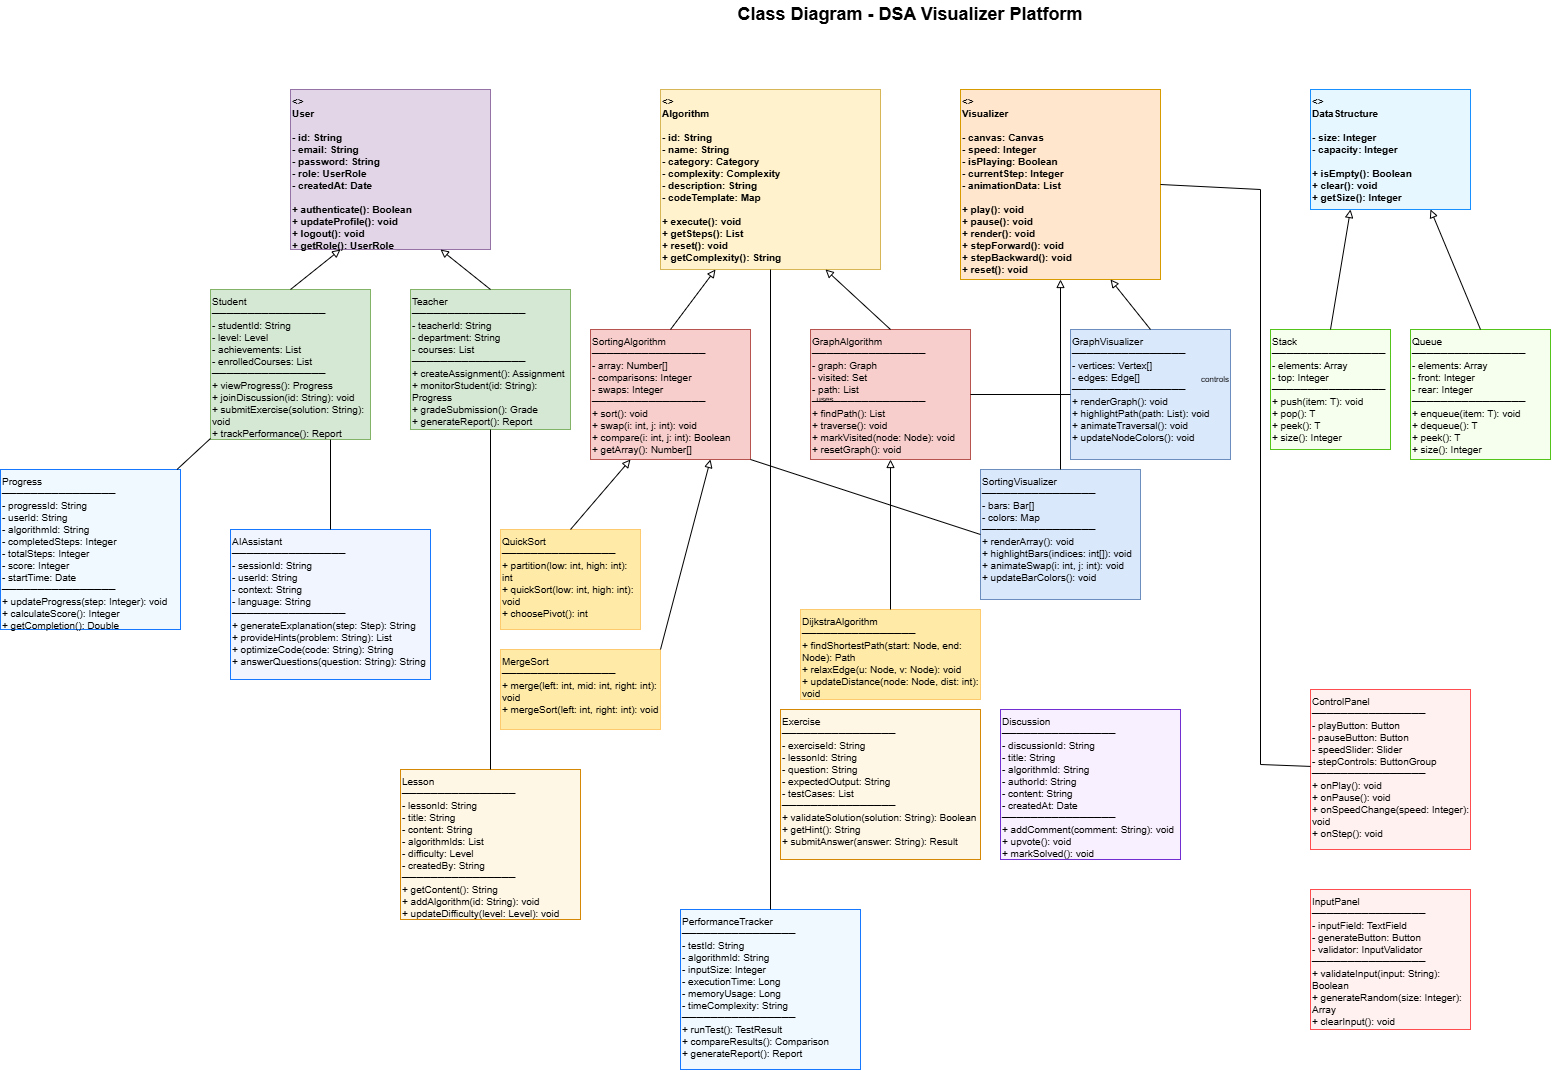
\includegraphics[width=1.0\textwidth]{enhanced-diagrams/class-diagram-clean.drawio}
\caption{Class Diagram cho Core Domain}
\label{fig:class-core}
\end{figure}

\subsubsection{User Management Classes}

\begin{itemize}
    \item \textbf{User}: Base class cho tất cả users
    \item \textbf{Student}: Extends User, thêm learning-specific attributes
    \item \textbf{Instructor}: Extends User, thêm teaching-specific attributes  
    \item \textbf{Admin}: Extends User, thêm system management capabilities
\end{itemize}

\subsubsection{Learning Domain Classes}

\begin{itemize}
    \item \textbf{Algorithm}: Represents thuật toán với metadata
    \item \textbf{Visualization}: Chứa animation data và configuration
    \item \textbf{LearningSession}: Tracks user interaction với algorithm
    \item \textbf{Progress}: Theo dõi learning progress của user
    \item \textbf{Assessment}: Quiz và evaluation system
\end{itemize}

\subsection{Service Layer Classes}
\label{subsec:service-classes}

\begin{figure}[H]
\centering
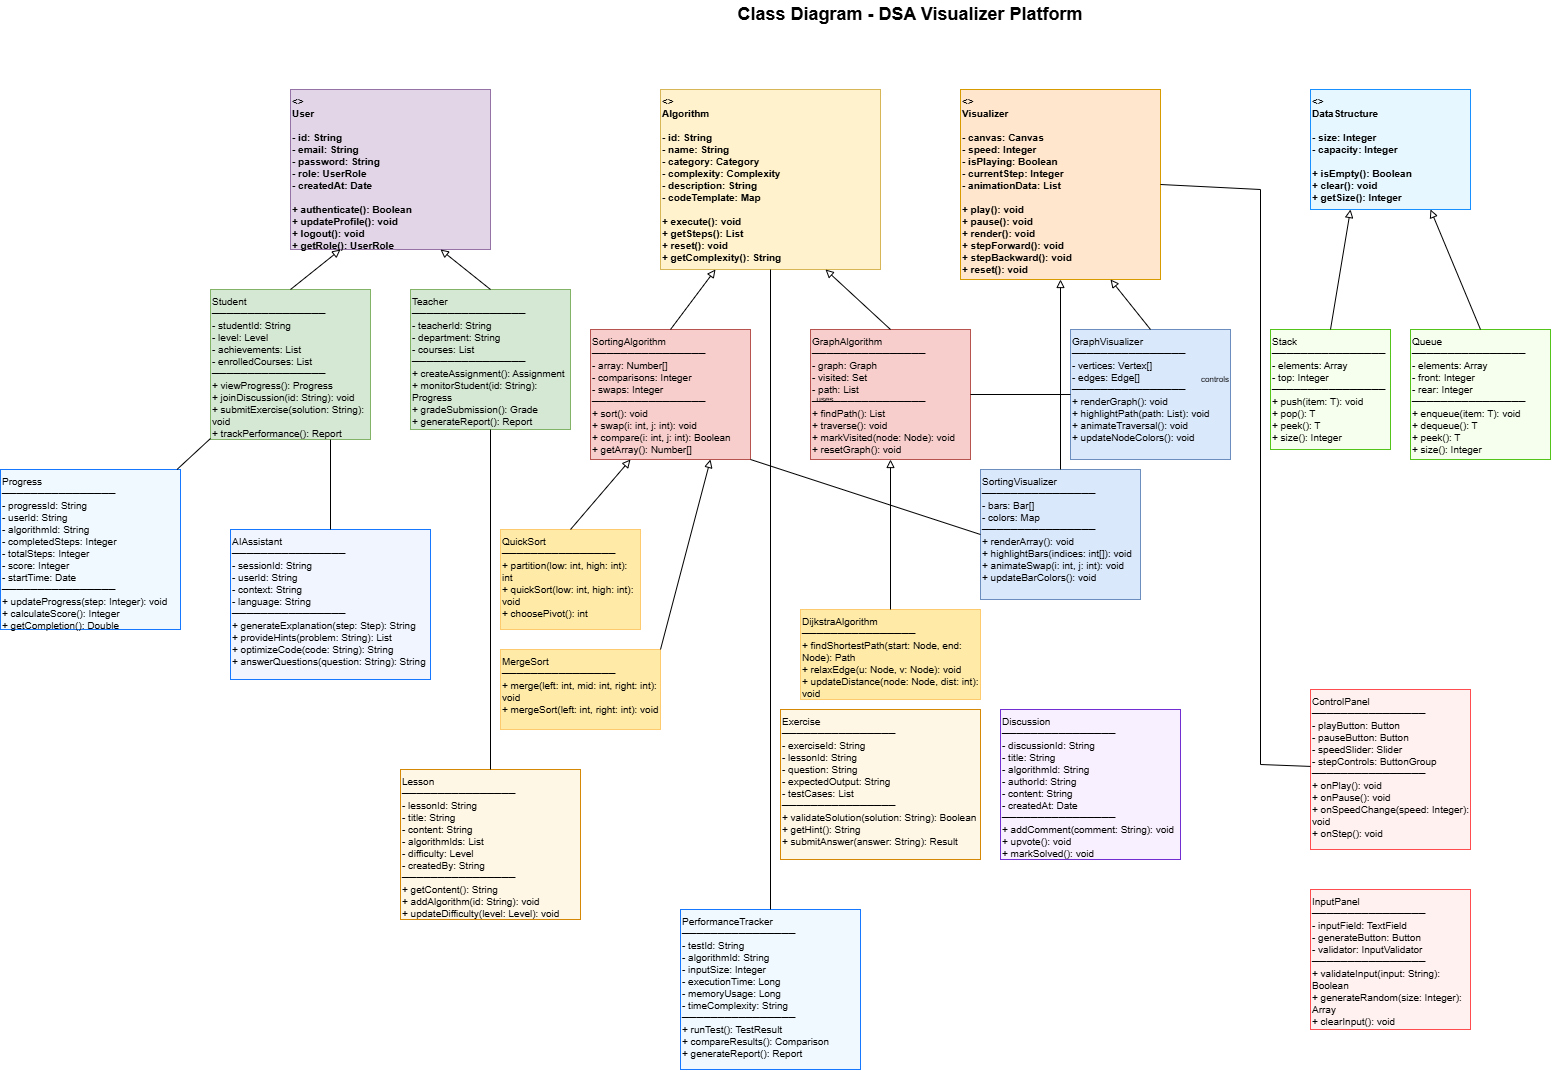
\includegraphics[width=1.0\textwidth]{enhanced-diagrams/class-diagram-clean.drawio}
\caption{Class Diagram cho Service Layer}
\label{fig:class-services}
\end{figure}

\subsubsection{Visualization Services}

\begin{itemize}
    \item \textbf{VisualizationEngine}: Core engine cho animation rendering
    \item \textbf{AnimationController}: Điều khiển animation playback
    \item \textbf{DataProcessor}: Xử lý input data cho visualization
    \item \textbf{RenderingService}: Abstract layer cho different renderers
\end{itemize}

\subsubsection{AI Services}

\begin{itemize}
    \item \textbf{AIAssistant}: Main interface cho AI interactions
    \item \textbf{OpenAIService}: Integration với OpenAI GPT
    \item \textbf{GeminiService}: Integration với Google Gemini
    \item \textbf{ContextBuilder}: Xây dựng context cho AI requests
\end{itemize}

\section{Activity Diagram}
\label{sec:activity-diagram}

\subsection{Learning Process Flow}
\label{subsec:learning-flow}

Activity diagram sau mô tả complete learning process từ khi student bắt đầu học một thuật toán mới:

\begin{figure}[H]
\centering
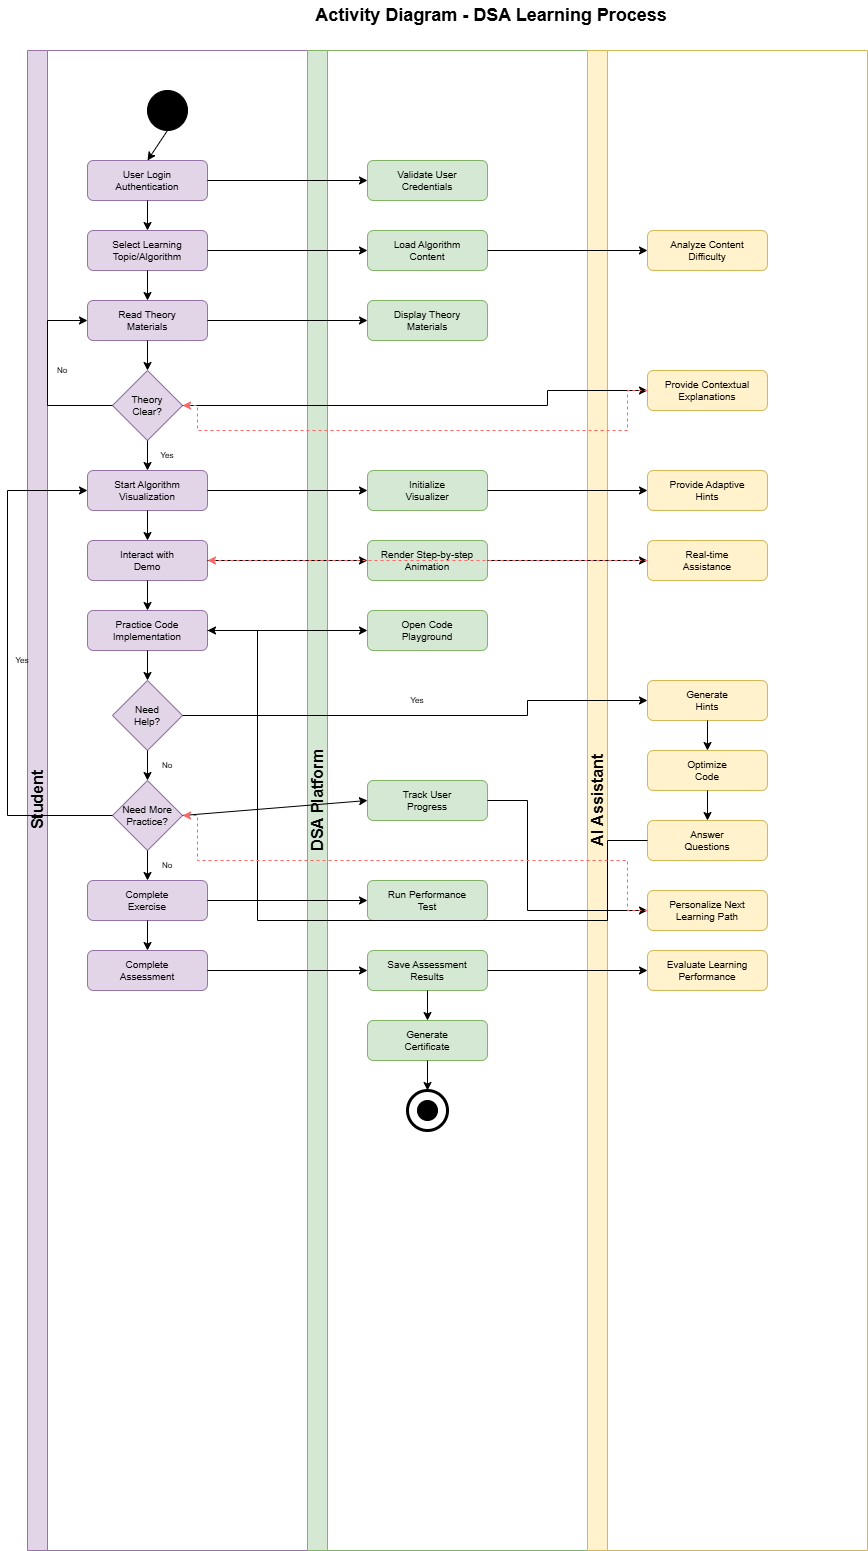
\includegraphics[width=0.8\textwidth]{enhanced-diagrams/activity-diagram-clean.drawio}
\caption{Activity Diagram cho Learning Process}
\label{fig:activity-learning}
\end{figure}

\subsubsection{Main Activities}

\begin{enumerate}
    \item \textbf{Algorithm Selection}: Student chọn thuật toán từ library
    \item \textbf{Theory Study}: Đọc theoretical background
    \item \textbf{Visualization Practice}: Tương tác với animated visualization
    \item \textbf{Code Understanding}: Phân tích implementation code
    \item \textbf{Problem Solving}: Áp dụng thuật toán vào bài tập
    \item \textbf{Assessment}: Đánh giá mức độ hiểu biết
    \item \textbf{Progress Update}: Cập nhật learning progress
\end{enumerate}

\subsubsection{Decision Points}

\begin{itemize}
    \item \textbf{Prerequisite Check}: Kiểm tra điều kiện tiên quyết
    \item \textbf{Difficulty Assessment}: Đánh giá độ khó phù hợp
    \item \textbf{Understanding Verification}: Xác nhận mức độ hiểu
    \item \textbf{Need Help Decision}: Quyết định có cần AI assistance
\end{itemize}

\subsection{AI Assistance Flow}
\label{subsec:ai-flow}

\begin{figure}[H]
\centering
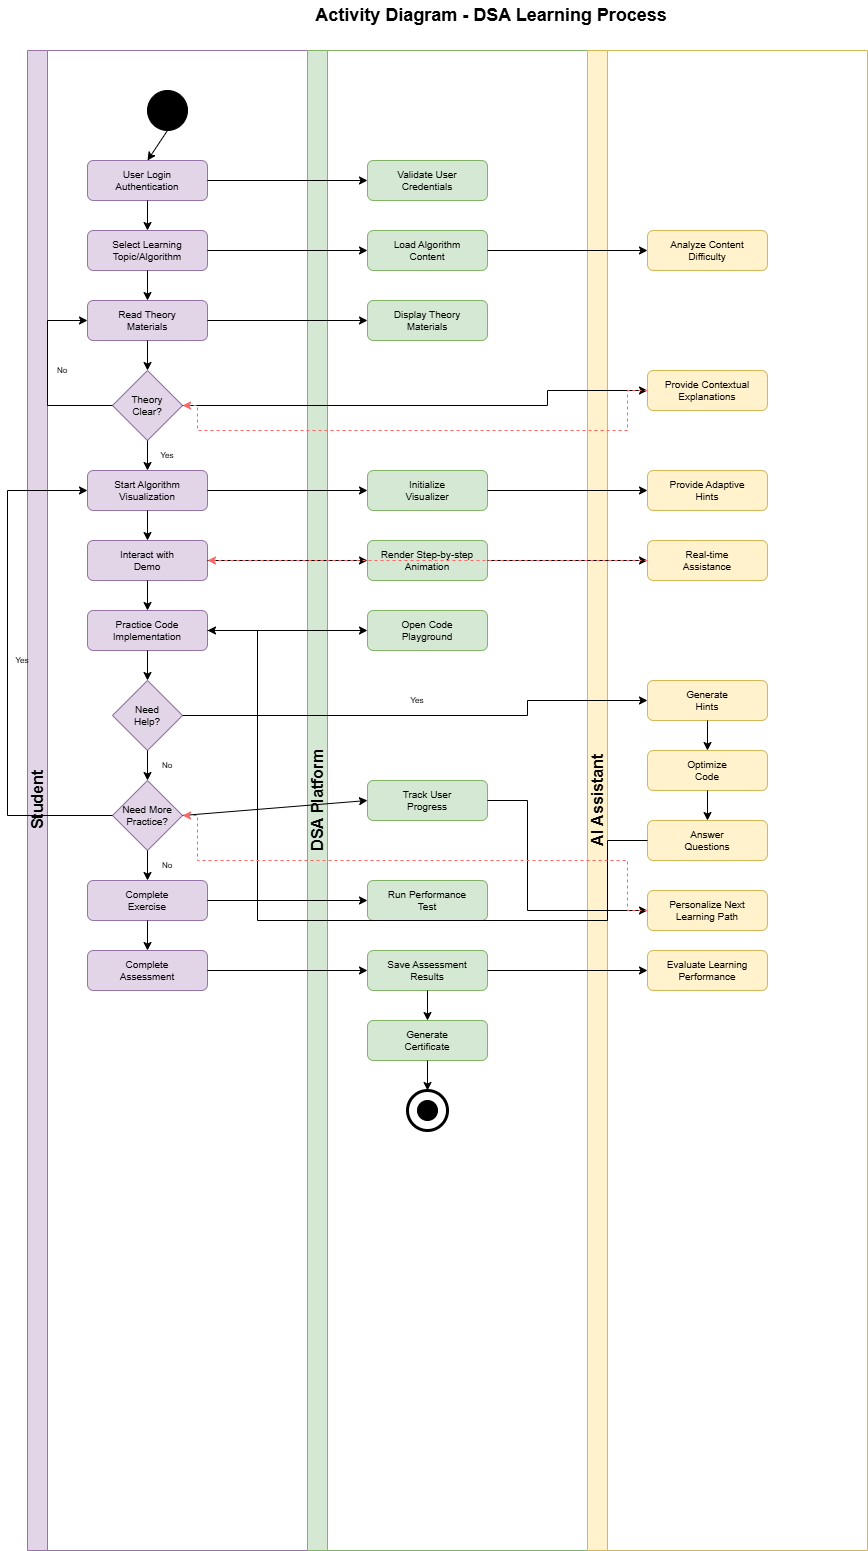
\includegraphics[width=0.7\textwidth]{enhanced-diagrams/activity-diagram-clean.drawio}
\caption{Activity Diagram cho AI Assistance Flow}
\label{fig:activity-ai}
\end{figure}

Process khi student request AI help:

\begin{enumerate}
    \item \textbf{Context Collection}: Gather current learning context
    \item \textbf{Query Processing}: Process natural language query
    \item \textbf{AI Model Selection}: Chọn appropriate AI model
    \item \textbf{Response Generation}: Generate contextual response
    \item \textbf{Response Formatting}: Format cho display
    \item \textbf{Feedback Collection}: Thu thập user feedback
\end{enumerate}

\section{Sequence Diagram}
\label{sec:sequence-diagram}

\subsection{Visualization Rendering Sequence}
\label{subsec:visualization-sequence}

Sequence diagram sau mô tả interaction giữa các components khi render visualization:

\begin{figure}[H]
\centering
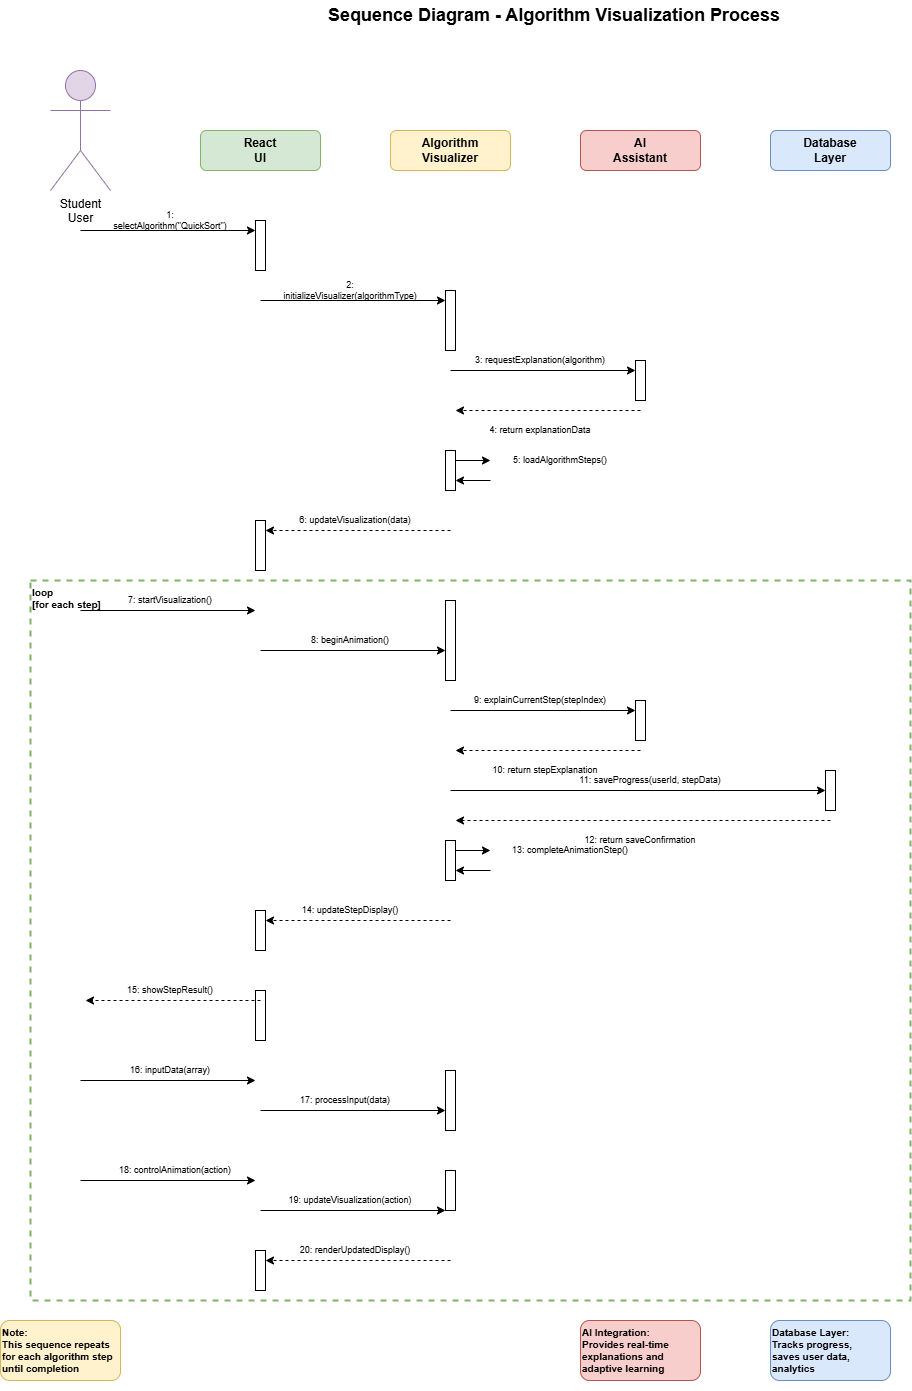
\includegraphics[width=1.0\textwidth]{enhanced-diagrams/sequence-diagram-clean.drawio}
\caption{Sequence Diagram cho Visualization Rendering}
\label{fig:sequence-viz}
\end{figure}

\subsubsection{Participants}

\begin{itemize}
    \item \textbf{Student}: User initiating visualization
    \item \textbf{VisualizationUI}: Frontend visualization component
    \item \textbf{VisualizationEngine}: Core rendering engine
    \item \textbf{AnimationController}: Animation management
    \item \textbf{DataProcessor}: Input data processing
    \item \textbf{ProgressTracker}: Learning progress tracking
\end{itemize}

\subsubsection{Key Interactions}

\begin{enumerate}
    \item Student selects algorithm và input parameters
    \item UI validates input và sends request to engine
    \item Engine processes data và prepares animation steps
    \item AnimationController manages playback timing
    \item Progress tracking updates throughout process
    \item Final state saved to user progress
\end{enumerate}

\subsection{AI Assistant Interaction Sequence}
\label{subsec:ai-sequence}

\begin{figure}[H]
\centering
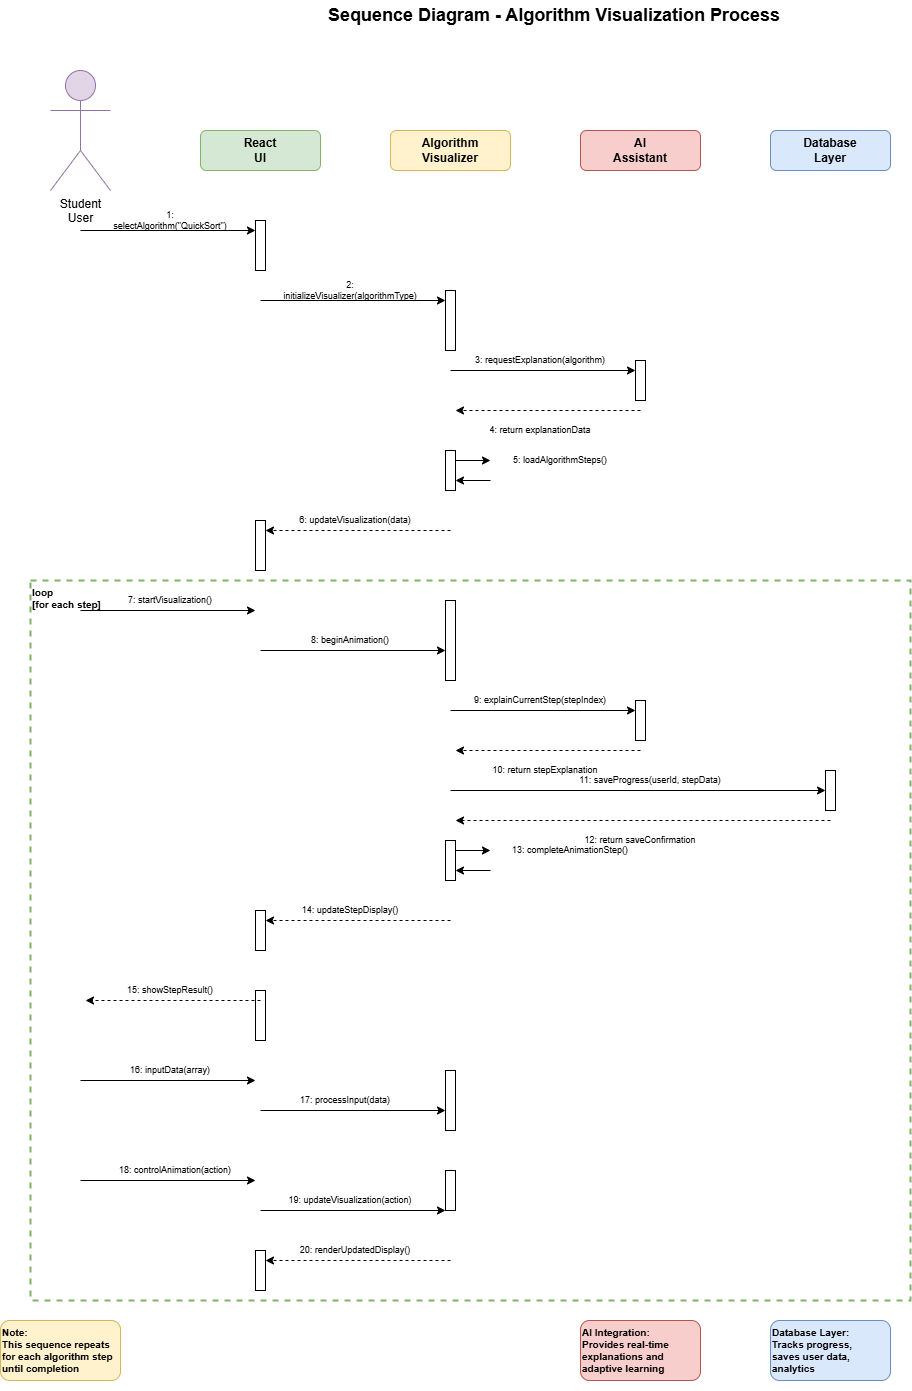
\includegraphics[width=1.0\textwidth]{enhanced-diagrams/sequence-diagram-clean.drawio}
\caption{Sequence Diagram cho AI Assistant Interaction}
\label{fig:sequence-ai}
\end{figure}

\subsubsection{Multi-Model AI Architecture}

Platform sử dụng multiple AI models để optimize cho different use cases:

\begin{enumerate}
    \item \textbf{OpenAI GPT}: Cho natural language explanations
    \item \textbf{Google Gemini}: Cho code generation và analysis
    \item \textbf{Context Router}: Intelligent routing dựa trên query type
    \item \textbf{Response Aggregator}: Combine responses từ multiple models
\end{enumerate}

\subsection{Community Interaction Sequence}
\label{subsec:community-sequence}

\begin{figure}[H]
\centering
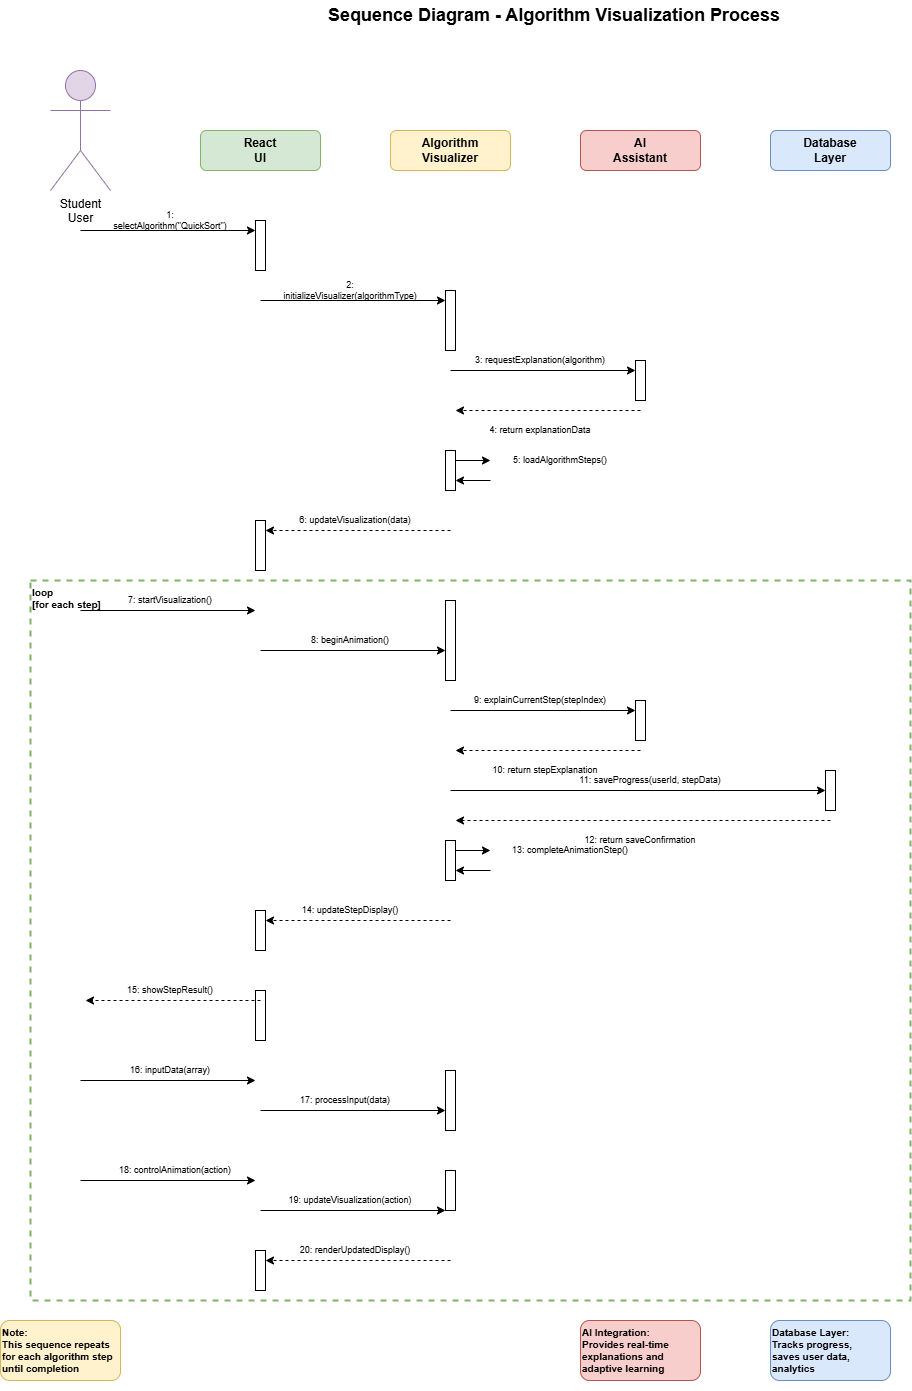
\includegraphics[width=1.0\textwidth]{enhanced-diagrams/sequence-diagram-clean.drawio}
\caption{Sequence Diagram cho Community Features}
\label{fig:sequence-community}
\end{figure}

Mô tả interaction trong forum và Q\&A system:

\begin{enumerate}
    \item User posts question hoặc discussion topic
    \item System validates content và applies moderation rules
    \item Notification service alerts relevant users
    \item Other users provide answers và comments
    \item Voting system ranks responses
    \item AI assistant có thể provide supplementary answers
    \item Final resolution updates knowledge base
\end{enumerate}
